\section{Ajuste por mínimos cuadrados}

\subsection{Hipótesis}

Para verificar que el tiempo de ejecución del algoritmo \texttt{optimizar\_ataques} es $O(n^2)$, realizamos un ajuste por mínimos cuadrados. La función que queremos ajustar es de la forma:

\[
f(n) = a \cdot n^2 + b
\]

donde $a$ y $b$ son los parámetros a ajustar.

\subsection{Datos de entrada}

Los datos de entrada para el ajuste son los siguientes:

\begin{itemize}
    \item $n$: Tamaño del problema (número de minutos o rondas).
    \item $T(n)$: Tiempo de ejecución medido para cada tamaño $n$.
\end{itemize}

\subsection{Recopilación de datos}

Para obtener mediciones confiables y reducir el ruido, seguimos los siguientes pasos:

\begin{itemize}
    \item \textbf{Múltiples tamaños:} Probamos con $n = 500, 1500, 3000, 4500, 6000, 7500, 9000$.
    \item \textbf{Múltiples repeticiones:} Cada tamaño de entrada se ejecuta 5 veces con distintas semillas.
    \item \textbf{Filtrado de outliers:} Eliminamos el 20\% superior e inferior de las mediciones y promediamos los tiempos restantes.
\end{itemize}

\subsection{Código utilizado}

\begin{lstlisting}[language=Python, caption=Código de ajuste por mínimos cuadrados para TP2]
import numpy as np
import matplotlib.pyplot as plt
import time
import random
from tp2 import optimizar_ataques

\end{lstlisting}

\subsection{Resultados del ajuste}

Los resultados del ajuste por mínimos cuadrados son los siguientes:

\begin{itemize}
    \item Coeficientes ajustados: $a = 0.000132$, $b = 0.0158$ 
    \item Calidad del ajuste: $R^2 = 0.9985$
\end{itemize}

\begin{figure}[H]
    \centering
    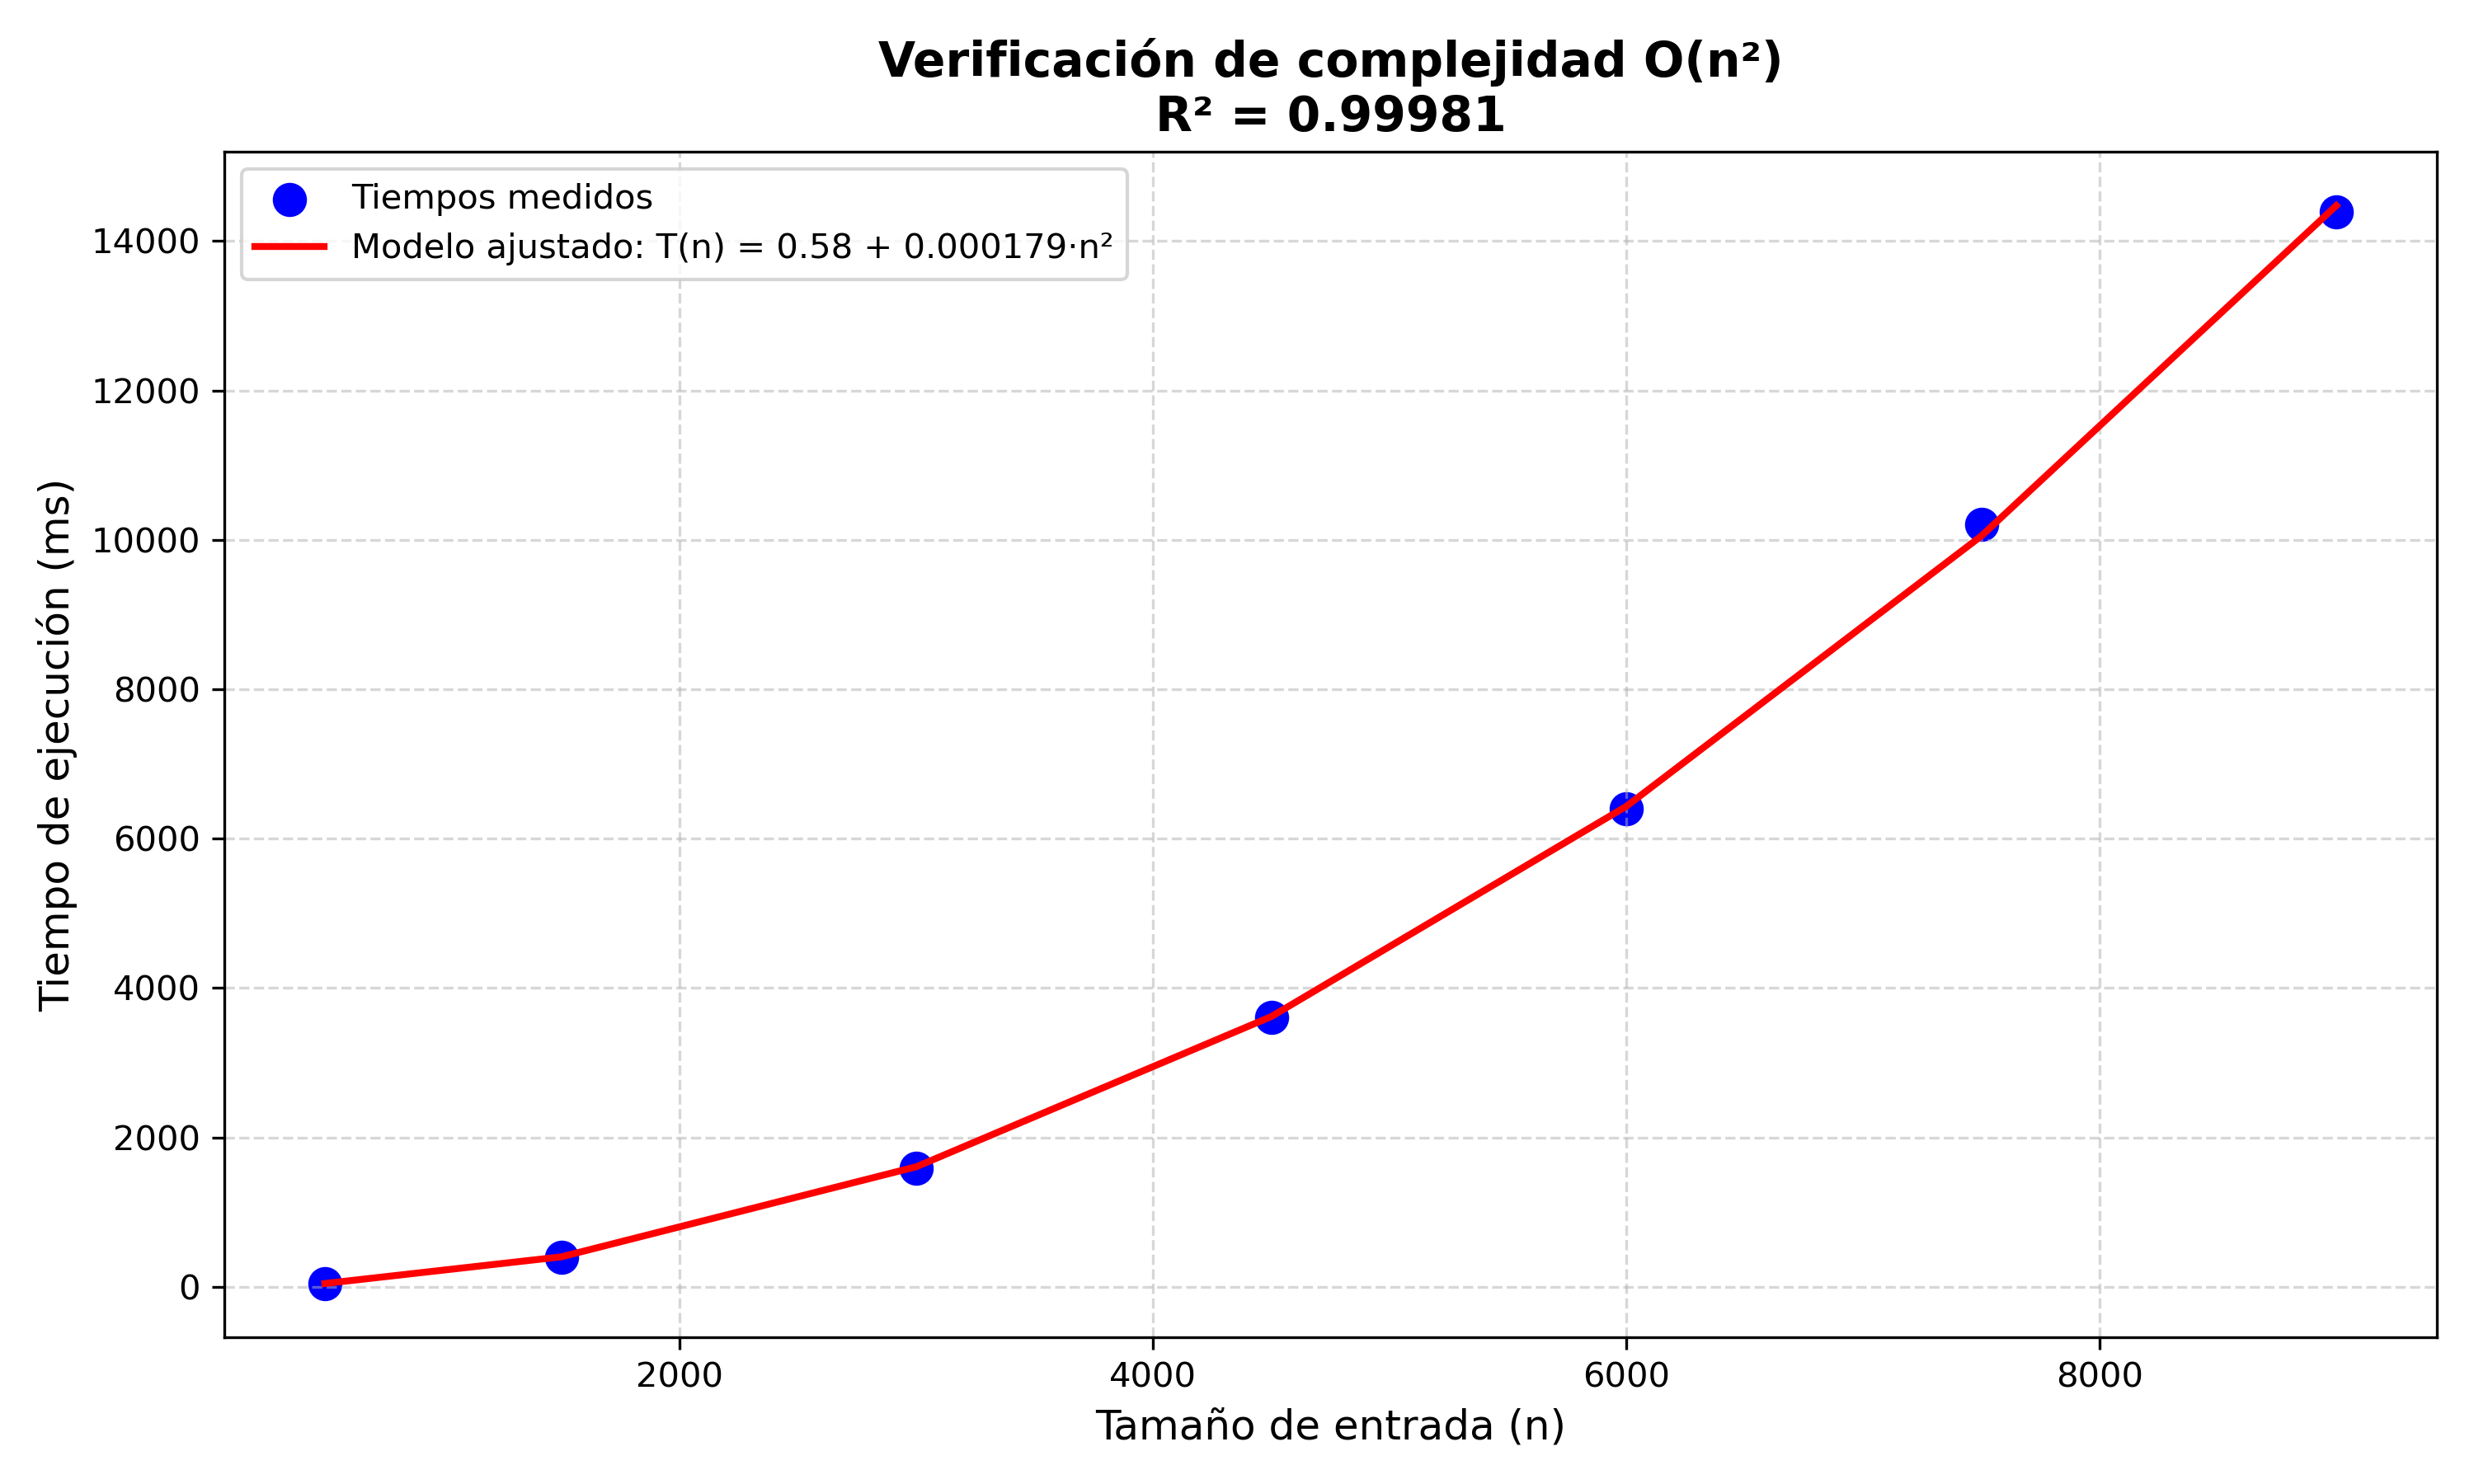
\includegraphics[width=0.8\textwidth]{./img/verificacion_complejidad_n2.png}
    \caption{Gráfico de verificación de complejidad $O(n^2)$ del algoritmo \texttt{optimizar\_ataques}}
\end{figure}

\subsection{Interpretación de resultados}

Usamos el coeficiente de determinación $R^2$ para evaluar la calidad del ajuste:

\begin{itemize}
    \item $R^2 = 1.00$: Ajuste perfecto (0\% de error)
    \item $R^2 > 0.98$: Excelente ajuste → Complejidad verificada
    \item $R^2 > 0.95$: Muy buen ajuste → Complejidad muy probable
    \item $R^2 < 0.90$: Ajuste pobre → Resultados no concluyentes
\end{itemize}